
\chapter{O \acl{IoT} no cultivo da Salicórnia}

 A \sr \space \textit{J. Woods (S. ramosissima)}\cite{JoaoSilva} que serve de mote a esta dissertação, é uma espécie do género \textit{Salicornia L.}, pertencente à família das beterrabas denominada de \textit{Chenopodiaceae}\cite{chenopodiaceae}.  Neste capítulo será apresentada a planta, as suas principais características e propriedades, bem como as suas diferentes aplicações medicinais e alimentares. Este capítulo servirá ainda como uma pequena introdução ao conceito de \ac{IoT} e à sua  importância no contexto deste projeto.


\section{Características da planta}


A Salicórnia é uma espécie halófita, adaptada a viver em ambientes com elevado teor de sal\cite{ferri}, sendo uma das mais evoluídas da sua família. É uma planta anual de dimensão pequena, aparentemente sem folhas, ereta, com caules carnudos e suculentos, simples e/ou extremamente ramificados, segmentados por articulações\cite{Silva2000}, geralmente com menos de 30 cm de altura\cite{overviewsal}. Esta planta tem uma coloração durante a maior parte do ano verde-escuro mas, no outono, a sua ramagem torna-se verde-amarelado ou mesmo vermelho-púrpura (figura \ref{primoutono})\cite{Silva2000}.





A Salicórnia desenvolve-se preferencialmente no litoral costeiro, em pântanos e sapais salgados ou em margens de salinas temporariamente alagadas. Encontra-se distribuída maioritariamente na parte oeste da Europa e a oeste da região do Mediterrâneo, sendo uma das espécies mais abundantes\cite{Figueroa1987}. Em Portugal, onde é vulgarmente conhecida como erva-salada, sal verde e/ou espargos do mar\cite{RaquelPinto}, é encontrada frequentemente nas margens dos canais da Ria de Aveiro e Ria Formosa (Algarve)\cite{RaquelPinto} sendo encontrada com menos frequência na região do Minho\cite{Silva2000}. 

\newpage

\begin{figure}[h]
	\centering
	\begin{minipage}[b]{0.49\textwidth}
		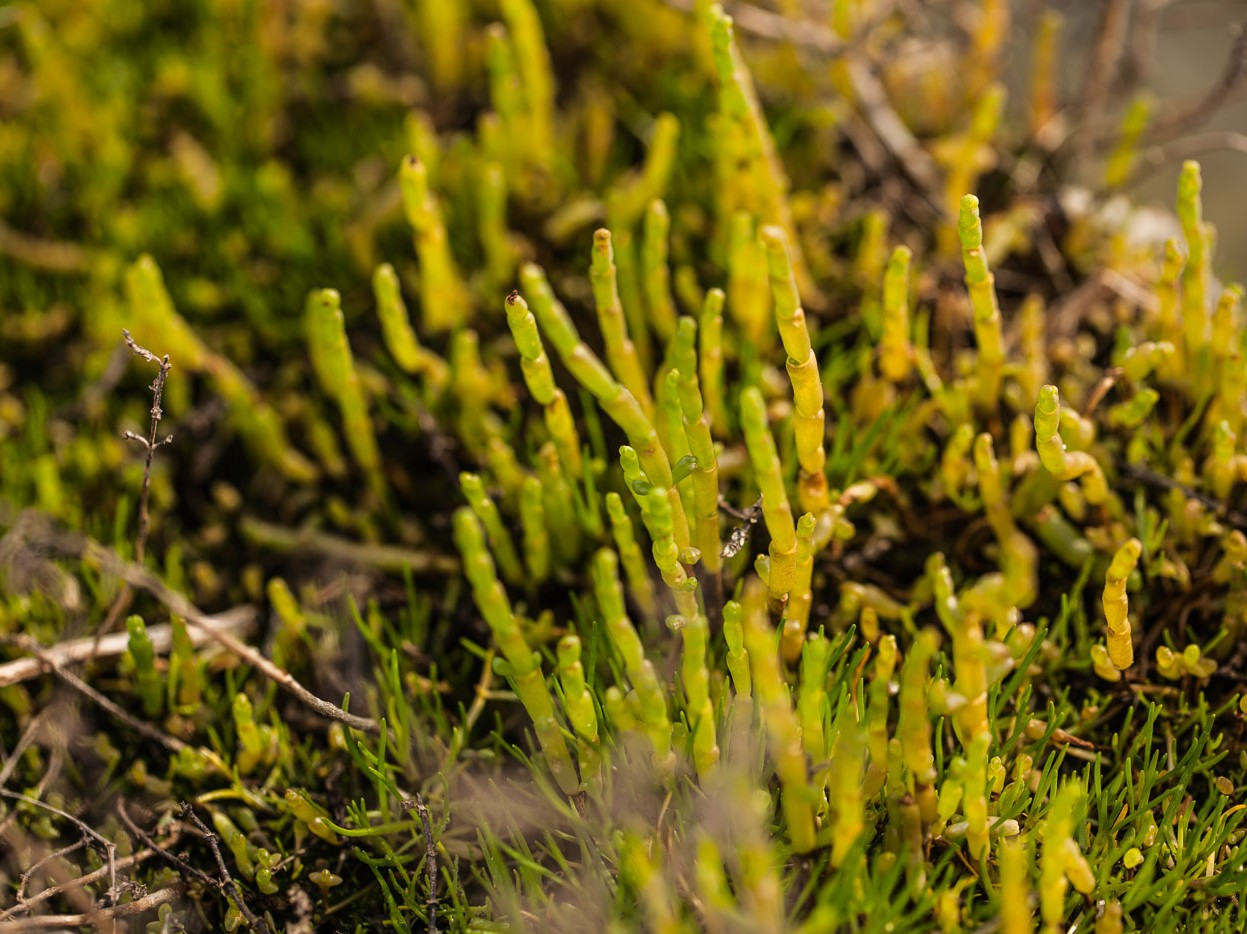
\includegraphics[width=\textwidth]{img/cap2-sali/Salicornia04.JPG}
	\end{minipage}
	\hfill
	\begin{minipage}[b]{0.49\textwidth}
		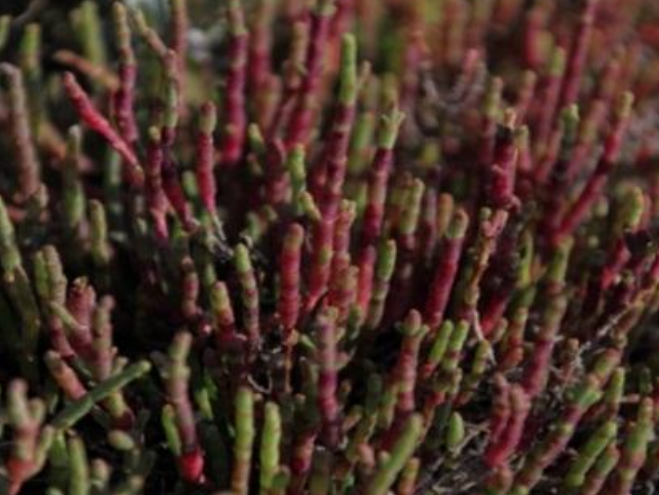
\includegraphics[width=\textwidth]{img/cap2-sali/sal-outono.png}
	\end{minipage}
	\caption[Coloração da planta \sr \space na primavera (à esquerda) e no outono (à direita)]{Coloração da planta \sr \space na primavera (à esquerda) e no outono (à direita) (Fotografias por José M. G. Pereira)}
	\label{primoutono}
\end{figure}



Esta planta é pouco estudada pelos cientistas\cite{Figueroa1987}, sabendo-se apenas que possui um ciclo de vida anual bem definido (figura \ref{ciclodevida}), com gerações discretas e as suas sementes são hermafroditas\cite{Silva2007}. A Salicórnia cresce habitualmente entre março, início da sementeira (A da figura \ref{ciclodevida}) com respetivo crescimento (B da figura \ref{ciclodevida}) e novembro fechando assim o ciclo com a produção de sementes (E da figura \ref{ciclodevida}). Entre maio  e agosto decorre a colheita da planta\cite{RaquelPinto} (C da figura \ref{ciclodevida}) que pode ser utilizada para os mais diversos fins. A floração ocorre fundamentalmente no mês de outubro\cite{Figueroa1987} (D da figura \ref{ciclodevida}). 



	
\begin{figure}[!htb]
	\centering
	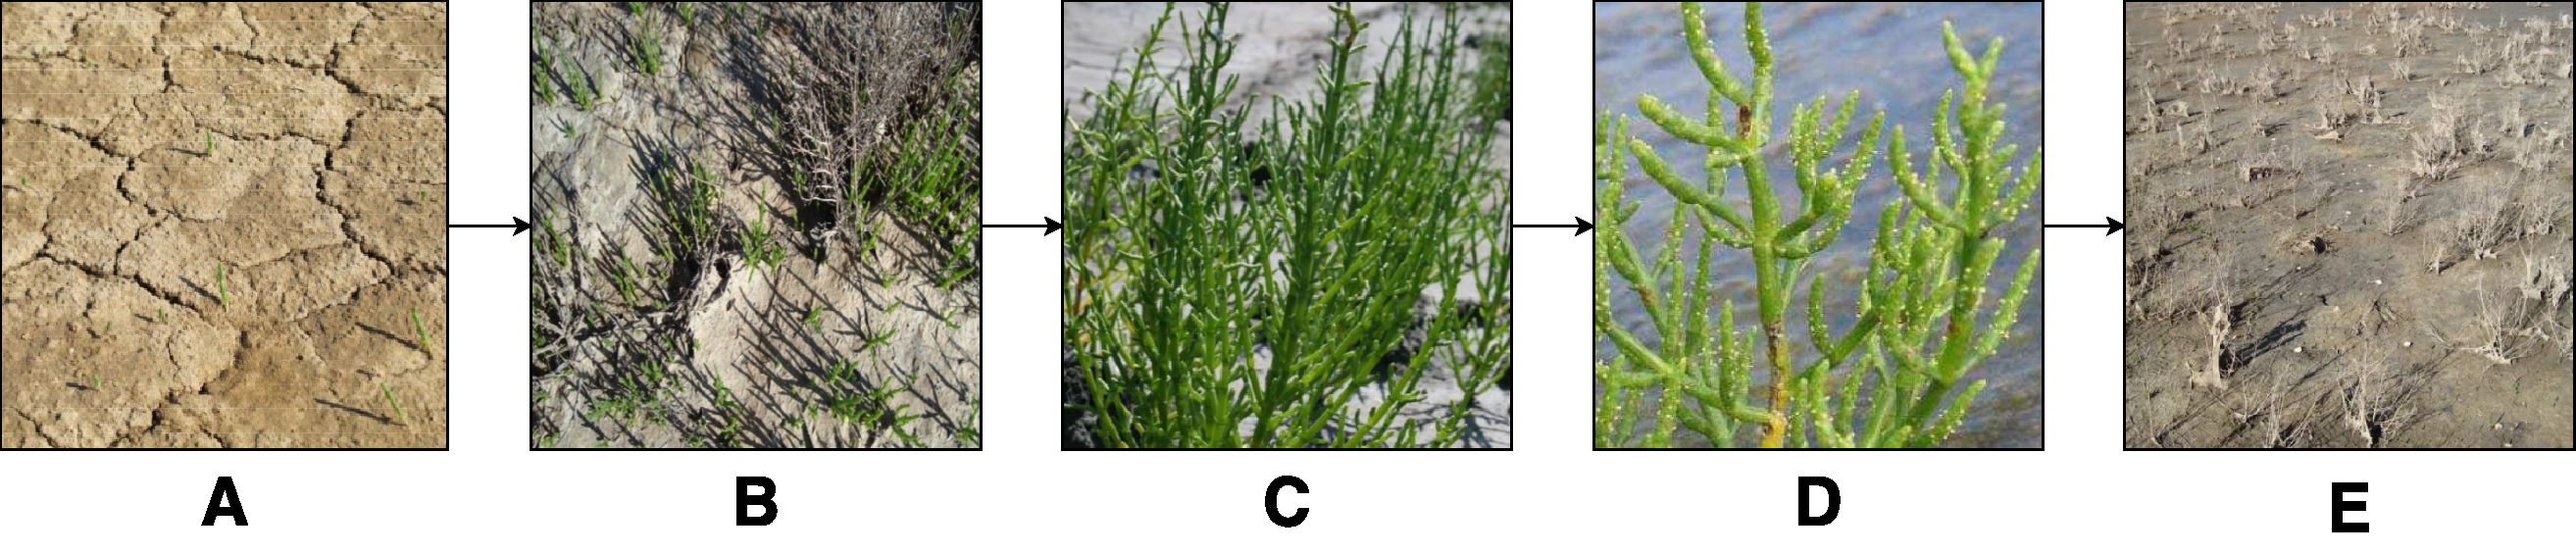
\includegraphics[width=\linewidth]{img/cap2-sali/ciclo/ciclodevida.pdf}
	\caption[Esquema representativo do ciclo de vida da \sr.]{Esquema representativo do ciclo de vida da \sr. A - semente incluída no sedimento; B -jovens plantas e plantas senescentes do ano anterior; C - planta no estado vegetativo, caule carnudo e articulado; D - planta no estado de floração; E - planta no estado senescente. (Fotografias por Helena Silva)}
	\label{ciclodevida}
\end{figure}



\section{Condições ideais de cultivo da Salicórnia}

O crescimento da Salicórnia é influenciado por diversos fatores ambientais que são atualmente estudados pelos biólogos, sendo a salinidade um dos mais importantes, já que influencia a distribuição, a abundância e a fisiologia da planta. Um estudo realizado por \textit{Silva et al.}\cite{Silva2007} comprova que esta planta halófita apresenta um crescimento ideal em salinidades baixas ou moderadas. Este estudo permite considerar ao contrário do que se pensava, esta planta como uma halófita não obrigatória, já que o seu crescimento ideal não acontece em condições de salinidade elevada, tal como se esperava. Embora o crescimento ideal ocorra a baixas salinidades, a Salicórnia é capaz de tolerar níveis elevados de sais\cite{Rubio-Casal2003}.

\section{Importância da planta}



Desde a antiguidade que as espécies do género \textit{Salicornia L.} estão incluídas na alimentação humana. Normalmente consome-se crua, cozinhada ou seca. Quando crua é usada como acompanhamento das mais diversas refeições enquanto que seca ou triturada é usada como especiaria, para tempero na confeção de peixes, marisco ou carnes. O sal verde, como é conhecida, é um grande substituto do sal comum, pois é rico em substâncias depurativas e diuréticas. Os seus caules carnudos são bastante requisitados para cozinhas \textit{gourmet}, não só pelo seu sabor salgado, mas também pelo seu elevado valor nutricional\cite{Filomena2009}, nomeadamente pelos níveis de minerais e vitaminas antioxidantes, como a  vitamina C e o $\beta$-caroteno. A Salicórnia é também uma fonte de proteínas e possui alto teor de ácidos gordos essenciais, destacando-se o  ómega-3\cite{Ventura2011}. A nível medicinal, existem diversos estudos que revelam as propriedades químicas da planta, tornam-na eficiente na prevenção e tratamento de algumas doenças, tais como, a hipertensão, cefaleias e escorbuto, diabetes, obesidade, cancro, entre outras\cite{Wang2012}.

Tendo em conta todas estas propriedades alimentares, medicinais e comerciais da Salicórnia, torna-se fulcral controlar o seu cultivo, a fim de otimizar a produção para tirar maior partido da sua importância biológica. Este controlo pode ser feito recorrendo à tecnologia, tal como será descrito nas próximas secções deste capítulo e ao longo do desenvolvimento desta dissertação.  



%alterar bastante o texto... palha














%a \sr que impulsionará toda esta dissertação. Serão descritas as principais características desta planta, principais propriedades e as diferentes aplicações alimentais existentes no mercado. 



\section{Evolução tecnológica: o \acl{IoT}}


Antes de descrever a importância e o conceito de \ac{IoT}, é necessário entender as diferenças entre os termos Internet e Web (\ac{WWW}), que são usados indistintamente pela sociedade. A Internet é a camada ou rede física composta por \textit{switches}, \textit{routers} e outros equipamentos. A sua principal função é transportar informações de um ponto para outro de forma rápida, confiável e segura. Por outro lado, a Web pertence à camada de aplicações que opera sobre a Internet cuja principal função é oferecer uma interface que transforme as informações que fluem pela Internet em algo útil\cite{Evans2011a}.


%Ao longo do tempo, a Web passou e continua a passar por várias etapas evolucionárias, identificadas como Web 1.0, Web 2.0 e Web 3.0. 

%\begin{itemize}
%	\item \textbf{Web 1.0 - passado}: esta primeira etapa foi inventada por Tim Berners Lee em 1989\cite{Getting}. Nesta fase surgiram os principais conceitos que conhecemos da Internet atual: \ac{URL}, \ac{HTML} e o \ac{HTTP}. Mais tarde, em 1998 foi criado por Larry Page e Sergey Brin o Google que criou simplicidade nas pesquisas na Web\cite{Lovato2014}. 
	
%	\item \textbf{Web 2.0 - presente}: a Web cresceu muito e muito rapidamente. Atualmente é considerada a versão mais próxima da visão de Tim Berners Lee (colaborativa), usado como meio de interação, comunicação global compartilhamento de informação. 
	
%	\item \textbf{Web 3.0 - futuro}: para o futuro prevê-se que os conteúdos \textit{online} possam vir a estar organizados de forma semântica, muito mais personalizados para cada utilizador, sites, aplicações inteligentes e/ou publicidade baseada nas pesquisas e nos comportamentos.
%\end{itemize}

%A  primeira evolução real da Internet foi o aparecimento do \ac{IoT}, que a transformou em algo sensorial, através da medição de diferentes parâmetros, como por exemplo a temperatura, a pressão, as vibrações, a iluminação, a humidade, o \textit{stress}, entre outras. Através destes parâmetros poderão surgiu novas aplicações com elevado potencial para melhorar significativamente a forma como a sociedade vive, aprende, trabalha e se diverte. 

%\begin{figure}[h]
%	\centering
%	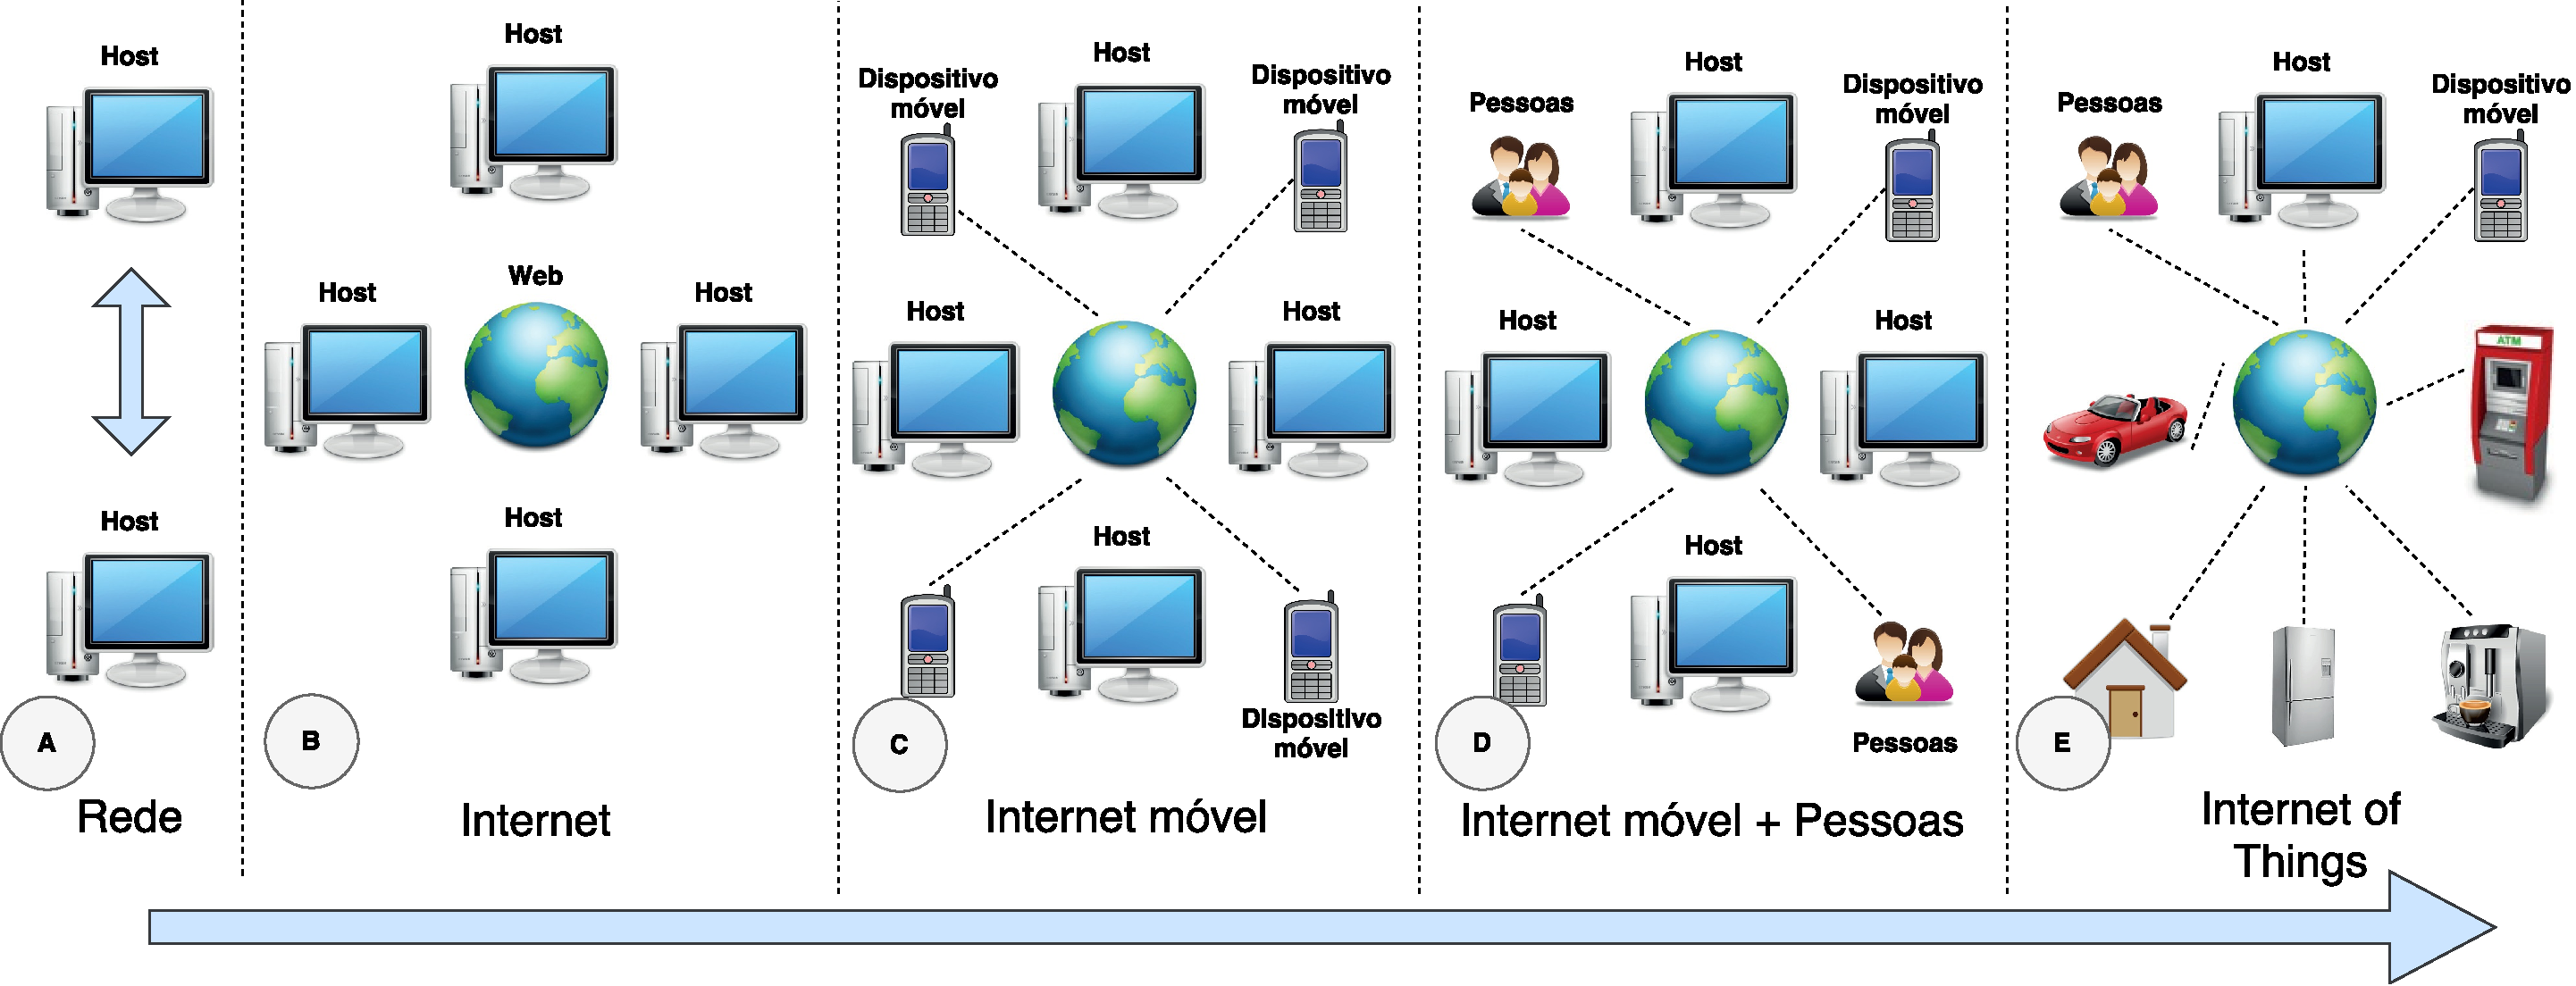
\includegraphics[width=\linewidth]{esquemas/iot-diagram.pdf}
%	\caption[Evolução da Internet em cinco fases]{ Evolução da Internet em cinco fases (Adaptado de \cite{Our2013})}
%	\label{iotEvolution}
%\end{figure}


%A figura \ref{iotEvolution} representa a evolução da Internet em cinco fases. Inicialmente surgiu a conexão entre dois computadores que permite a criação de uma rede (A da figura \ref{iotEvolution}), posteriormente nasce o conceito de \ac{WWW} ligando um grande número de computadores entre si (B da figura \ref{iotEvolution}). Seguidamente, surgiu a Internet móvel (C da figura \ref{iotEvolution}) que permitiu ligar dispositivos móveis à Internet, possibilitando a ligação da sociedade através das redes sociais (D da figura \ref{iotEvolution}).
%Finalmente, a Internet está a evoluir para o \ac{IoT}, permitindo ligar objetos do quotidiano ao sistema global de redes de computadores (E da figura \ref{iotEvolution})\cite{Our2013}.









%Uma das principais vantagens do \ac{IoT} é permitir ligar qualquer objeto eletrónicos à Internet passando este a ser controlado e gerido através da Internet. O volume de dados gerado por este tipo de ligação pode ser interpretado pelo modelo \ac{DIKW}\cite{Rowley2007}. Este modelo, também conhecido como pirâmide do conhecimento (figura \ref{dikw1}), é uma hierarquia informacional utilizada especialmente nas áreas da ciência da informação e na gestão do conhecimento, onde cada camada acrescenta certos atributos sobre a anterior.


%\begin{figure}[!htb]
%	\centering
%	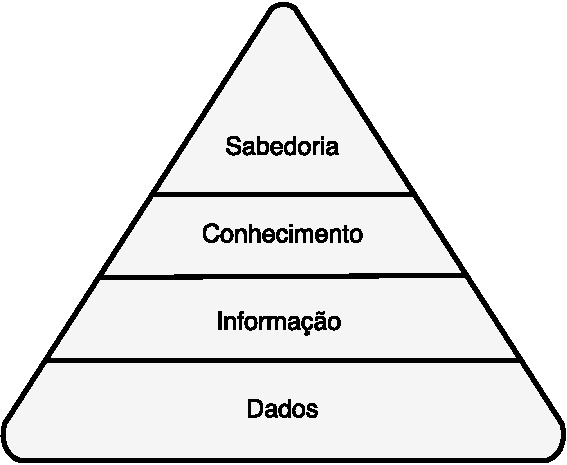
\includegraphics[scale=0.8]{img/cap3-iot/dikw.pdf}
%	\caption{Pirâmide do conhecimento: modelo DIKW}
%	\label{dikw1}
%\end{figure}



%A ligação dos objetos à Internet acarreta benefícios visíveis à nossa sociedade, possibilitando um maior controlo e entendimento de como os sistemas interagem entre si e proporcionando uma melhor qualidade de vida a todos. Embora as vantagens se sobreponham às desvantagens não nos podemos esquecer que existem alguns problemas a nível segurança, privacidade, legislação e identidade.



Com o avanço contínuo da tecnologia, surgiu o conceito de \ac{IoT}, em português Internet das Coisas. O \ac{IoT} engloba todos os dispositivos inteligentes que se encontram ligados à Internet e que conseguem ligar-se a outros dispositivos sem intervenção humana, utilizando a comunicação do tipo máquina-máquina (M2M). Isto é, permite que um dispositivo sem fios ou com fios, possa comunicar com outros dispositivos que possuam a mesma capacidade. Este método possibilita a captura de dados e consequente análise/processamento transformando-os em informação útil\cite{Li2015}. 

	O IoT tem evoluído continuamente sendo alvo de pesquisas onde as oportunidades são infinitas. O seu início remete ao ano de 1982, quando uma máquina de refrigerantes foi modificada e ligada à Internet, possibilitando o envio de alertas (quantidade de bebidas e grau de refrigeração) aos seus utilizadores\cite{Farooq2015}. Em 1999, Kevin Ashton propôs o termo "Internet das coisas" para descrever um sistema de dispositivos interligados\cite{KevinAshton}. Este conceito tem evoluído de tal forma que até ao final de 2020, prevê-se que sejam ligados 24 mil milhões de dispositivos à Internet no âmbito do \acl{IoT}\cite{Rivera2014}. Na figura \ref{libelimaplic} são apresentadas algumas das áreas de interesse do \ac{IoT}\cite{Gubbi2013}. 
	

\begin{figure}[!htb]
	\centering
	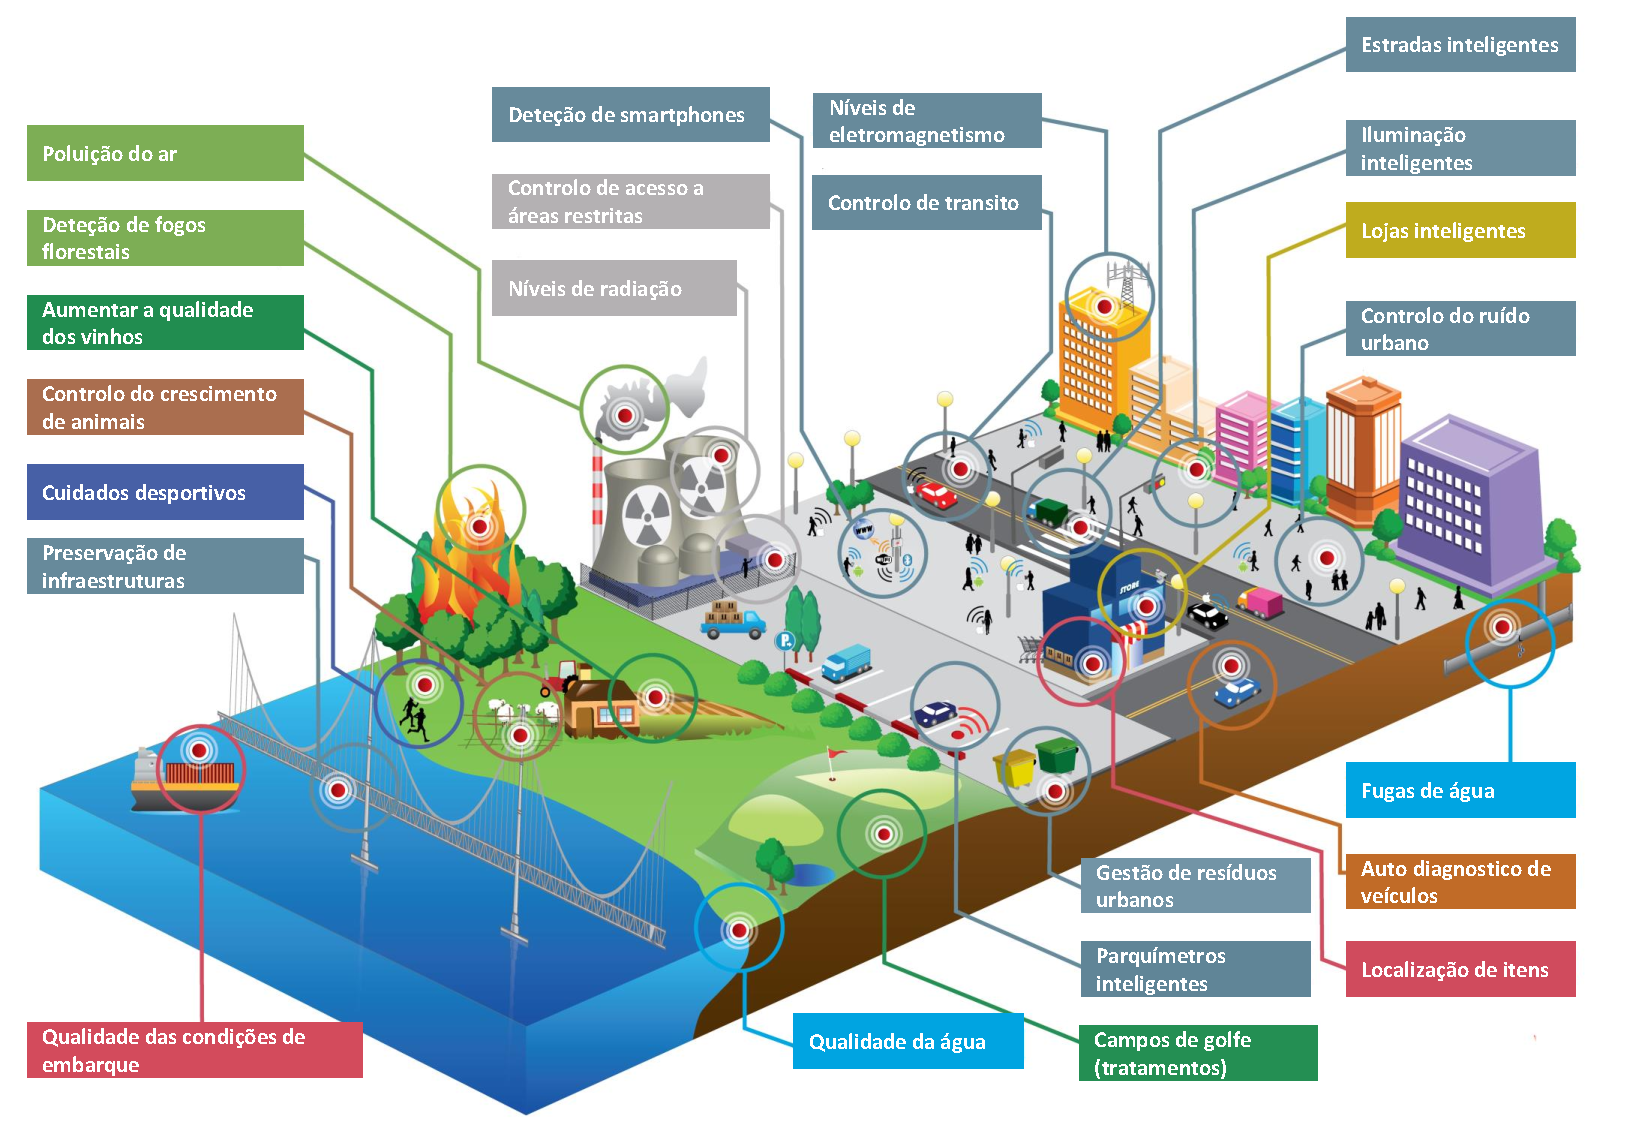
\includegraphics[width=\linewidth]{esquemas/adaptacaoiot.pdf}
	\caption[]{Áreas de interesse do \ac{IoT} (Adaptado de \cite{Gubbi2013})}
	\label{libelimaplic}
\end{figure}


Neste contexto, existem várias tecnologias que podem ajudar no desenvolvimento em larga escala do IoT, permitindo a recolha de informação, automatização de ações, controlo remoto, entre outros\cite{Farooq2015}. São exemplo as seguintes tecnologias: 

\begin{itemize}
	\item \ac{RFID}: é uma tecnologia de chave que torna os objetos identificáveis de forma exclusiva. Consiste num \textit{microchip} transcetor semelhante a um adesivo que pode ser ativo ou passivo, dependendo do tipo de aplicação. O seu tamanho e custo são reduzidos sendo facilmente integrado em qualquer objeto. 
	  
	\item \ac{WSN}: consiste numa rede de sensores bidirecional (sem fios) de forma\textit{ multi-hop}. É construída a partir de vários nós dispersos permitindo a recolha de dados específicos do objeto, que são processados e enviados para uma antena (\textit{gateway}). 
	
	\item Computação em nuvem (\textit{Cloud Computing}): com o aumento do número de dispositivos no âmbito do IoT, pensa-se que a \textit{cloud} será a única tecnologia capaz de analisar e armazenar todos os dados de forma eficaz. Consiste numa tecnologia de computação inteligente onde é possível processar, armazenar, analisar e disponibilizar dados.   
	
	\item Tecnologias de rede: têm um papel importante no sucesso do IoT, uma vez que são responsáveis pela ligação dos diferentes objetos. A tecnologia escolhida para este conceito tem de ser rápida e eficaz para conseguir lidar com uma grande quantidade de dispositivos. Alguns dos exemplos destas tecnologias são: rede 3G, 4G, Bluetooth e Wifi. 
	
\end{itemize}



Tendo em conta que a maioria das aplicações inteligentes já existentes no mercado não estão ligadas entre si, não se consegue tirar maior proveito do IoT. Neste sentido, têm surgido aplicações inovadoras e autónomas que melhoram significativamente a vida do ser humano\cite{Farooq2015}. De seguida, são apresentados três exemplos em que esta situação é visível. 


\begin{itemize}
	\item \textit{Smart Environment}: a previsão de desastres naturais (inundações, incêndios, terremotos, etc.) será possível devido às tecnologias inovadoras do IoT, e, para além disso, permite a monitorização adequada da poluição do ar no meio ambiente\cite{Farooq2015}.
		
	\item \textit{Smart Agriculture}: permite monitorizar a quantidade de nutrientes existente no solo, a intensidade da luz e a percentagem de humidade, melhorando o crescimento do cultivo agrícola através do ajuste automático da temperatura, da irrigação e da distribuição de fertilizantes\cite{-2013}.
	
	\item \textit{Smart Home}: possibilita o controlo remoto de determinados aparelhos nas nossas casas conforme as nossas necessidades. Para além disso, é possível monitorizar a energia gasta e o abastecimento de água possibilitando economizar recursos\cite{Farooq2015}. 
	 
\end{itemize}


A ligação dos objetos à Internet acarreta benefícios visíveis à nossa sociedade, possibilitando um maior controlo e entendimento de como os sistemas interagem entre si e proporcionando uma melhor qualidade de vida à população. Embora as vantagens se sobreponham às desvantagens não nos podemos esquecer que ainda existem alguns problemas a nível segurança, privacidade, legislação e identidade.


\section{Considerações finais}


Como vimos neste capítulo, as propriedades alimentares e terapêuticas da Salicórnia têm conduzido a um elevado interesse económico e ao aumento do seu valor comercial. Existem inúmeras empresas a cultivar esta espécie para que possa ser comercializada para os mais diversos fins, sendo que grande parte já é exportada. Uma vez que a Salicórnia carece de um controlo minucioso de certos parâmetros durante o seu cultivo, sendo estes ainda estudados pelos biólogos, existe necessidade de criar um sistema de monitorização, permitindo assim melhorar e conhecer as condições de produção desta espécie. O universo do \ac{IoT} pode ser aplicado neste contexto, uma vez que possibilita a interligação de equipamentos eletrónicos que melhorem a eficiência de produção de Salicórnia através da aplicação de sensores e atuadores no campo.  





